% Section content template for individual Educative lessons
% This file contains the actual content for a specific section
% Generated from Educative API section content

% Section: Behavioral Design Patterns
% Section ID: 5765883666628608
% Section Slug: behavioral-design-patterns
% Generated: 2025-12-11T06:16:26.910420

\subsection{What are behavioral patterns?}\label{D5iyYQKdGeZVvn2azZddT}
\\
\textbf{Behavioral design patterns} define how objects communicate and collaborate to accomplish tasks within a system. These patterns focus on effective interaction and responsibility-sharing among objects, without requiring significant changes to their internal code. This approach makes software systems more flexible, easier to maintain, and adaptable to future requirements.
\\
For example, while designing a notification system, we might want to send an email, a push notification, or a text message whenever a new blog post is published. Instead of writing separate code for each type, we can use the observer pattern, which automatically updates all notification services when something new happens. If we decide to add a Slack message later, we simply introduce a new observer---no changes are needed in the main publishing code.
\\
Several well-known behavioral design patterns exist. The most common patterns include Chain of Responsibility, Command, Iterator, Mediator, Observer, Visitor, Interpreter, Memento, State, Strategy, and Template Method. This lesson will explain the most important and commonly used patterns to help build a strong understanding of practical design and interview preparation.
\\
The illustration below shows all the patterns that fall under this category:

\begin{figure}[htbp]
 \centering
 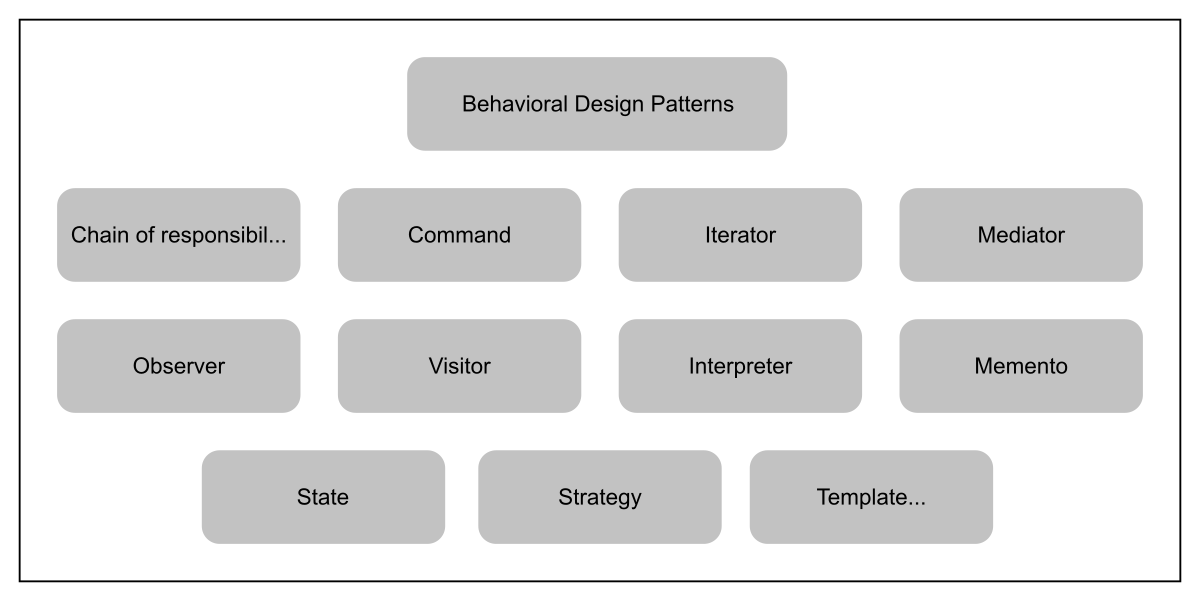
\includegraphics[width=0.5\textwidth]{Images/chapter_5/section_5765883666628608/4544552386822144.png}
 
\end{figure}

\subsection{Chain of Responsibility pattern}\label{1cs9bujrWRGy2RrXEgo1p-2}
\\
The \textbf{Chain of Responsibility} \textbf{pattern} allows a request sent by a client to be received by more than one object. It creates a chain of loosely-coupled objects that, upon receiving the request, either handle it or pass it to the next handler object.
\\
A common example of this pattern is~event bubbling~in~the DOM. An event propagates through different nested elements of the DOM until one of them handles it.

\subsection{Command pattern}\label{DxL45g0fl9E57Wk4GZZMO}
\\
The~\textbf{Command pattern}~allows encapsulation of the requests or operations into separate objects. It decouples the objects that send requests from those responsible for executing them.
\\
Consider an example where the client is accessing the methods of an API directly throughout the application. What will happen if the implementation of that API changes? The change will have to be made everywhere the API is being used.~To avoid this, we could use abstraction and separate the objects requesting from those implementing the request. Therefore, only the object making the call will need to change if a change occurs.

\subsection{Iterator pattern}\label{yoV97XQWhoDp_gBajKetd}
\\
The \textbf{Iterator pattern} allows the definition of various types of iterators that can sequentially iterate a collection of objects without exposing the underlying form.
\\
Iterators encapsulate how the traversal occurs in an iteration. Most languages have built-in iterators such as IEnumerable andIEnumerator. Iterators follow the behavior where they call a \texttt{next} function and step through a set of values until they reach the end. To do this, they need to maintain a reference to the current position and the collection they are traversing. Hence , an iterator has functions such as \texttt{next}, \texttt{hasNext}, \texttt{currentItem}, and\texttt{each}.

\subsection{Mediator pattern}\label{ZT1Io2XlXrg5iqU_Mn_zZ}
\\
It is a behavioral pattern that allows a \textbf{mediator} (a central authority) to act as the coordinator between different objects instead of the objects referring to each other directly. As the name implies, a mediator is a central authority through which various components can communicate. It allows the loose coupling of objects.
\\
A real-life example is a chat application. Here, the chat box acts as the mediator through which various users interact with one another.

\subsection{Observer pattern}\label{nJWyih8BoOtDGtLNh4Y1a}
\\
The \textbf{Observer pattern} is an important behavioral design pattern. It allows objects (observers) who have subscribed to an event to wait for input and react when notified. Therefore, they don't have to continuously check whether the input has been provided. The main subject maintains a list of all the observers, and whenever the event occurs, it notifies the observers so they can update their states accordingly.
\\
Let's look at a real-life example to map to this pattern. Consider a website that posts interesting articles. Every day, you visit the site to check for new articles; if there are none, you revisit after some time. What if you get a subscription to the website instead? Once you have the subscription, you'll be notified whenever a new article is posted. So now, instead of checking the site every few hours, you just wait for the notification about a new article.

\subsection{Visitor pattern}\label{-Vh30QfY21ofCt-DrloW9}
\\
The \textbf{Visitor pattern} allows the definition of new operations on the collection of objects without changing the objects' structure. This allows us to separate the class from the logic it implements.
\\
The extra operations can be encapsulated in a visitor object. The objects can have a visit method that accepts the visitor object. The visitor can then make the required changes and perform the operations on the received object. This allows the developers to make future extensions, extend the libraries/frameworks, etc.

\subsection{Interpreter pattern}\label{o0ok-Ki2ejHM8Dg0sMstK}
\\
The \textbf{Interpreter pattern} provides a way to interpret or translate sentences in a simple language using a set of interpreter objects. Each interpreter object represents a rule or part of the language grammar. Together, these objects can read, understand, and process statements. This pattern is helpful when defining and processing simple languages or expressions.
\\
A real-life example is a simple calculator. Here , we can create different \texttt{Expression} objects like \texttt{NumberExpression} for numbers and \texttt{AddExpression} or \texttt{SubtractExpression} for operations. Each expression object knows how to interpret itself and returns a result.

\subsection{Memento pattern}\label{WwSeTB98GMR-03TWka7fe}
\\
The \textbf{Memento pattern} captures and externalizes an object's internal state so that it can be restored to this state later without violating encapsulation. This pattern is commonly used to implement undo/redo functionality.
\\
This pattern uses three types of objects:~

\begin{enumerate}
\item
\protect\phantomsection\label{Stk1xOMWP1HVjMzGGLFi-}
\textbf{Originator:} The object whose state needs saving/restoring
\item
\protect\phantomsection\label{7MQyX0p007wFipetkgaTL}
\textbf{Memento:} The object that stores the state
\item
\protect\phantomsection\label{7kIYPs3IxjnnCBE5UsgxJ}
\textbf{Caretaker:} The object that requests and holds mementos, but does not modify them
\end{enumerate}
\\
For example, in a text editor, the \texttt{TextEditor} object is the \texttt{Originator}. When we want to save our work, the \texttt{TextEditor} creates a Memento object that stores the current text. The History\ object is the \texttt{Caretaker}. It keeps a list of Memento objects so we can undo changes. If we want to undo, the \texttt{TextEditor} asks for the last Memento and restores its state.

\subsection{State pattern}\label{0BjR5YSu3eD8dc5Cn_I0I}
\\
The \textbf{State pattern} lets an object change its behavior when its internal state changes. We create different state objects instead of using many \texttt{if} or \texttt{switch} statements. The main object keeps a reference to its current state object and passes work to it. Each state object defines how to handle actions for that state.
\\
For example, in a music player, the \texttt{MusicPlayer} object can be in a \texttt{PlayingState} or a \texttt{PausedState}. When we press the play/pause button, the \texttt{MusicPlayer} asks its current state object what to do. If it is in \texttt{PlayingState}, the state object will pause the music and change the state to \texttt{PausedState}. If it is in \texttt{PausedState}, the state object will play the music and switch back to \texttt{PlayingState}.

\subsection{Strategy pattern}\label{AnknGPq_ByyXPFztuxdE6}
\\
The \textbf{Strategy pattern} allows us to define a family of related algorithms and put each in its strategy object. A context object holds a reference to a strategy object and delegates the work to it instead of handling the logic directly. This pattern makes changing an algorithm at runtime easy without changing the main object's code.
\\
A real-life example is a navigation application. Here , the \texttt{NavigationApp} object acts as the context and selects a \texttt{RouteStrategy} object, such as \texttt{FastestRoute}, \texttt{ShortestRoute}, or \texttt{ScenicRoute}, to calculate the route. The navigation app can switch to a different strategy at any time to find a route in another way.

\subsection{Template Method pattern}\label{AY7ctycbNX13kCA3AFRCN}
\\
The \textbf{Template Method} \textbf{pattern} defines the basic steps of an algorithm in a base class, with some steps fixed and others left for subclasses to fill in. This lets us keep the process's common structure in one place while allowing parts to vary when needed. It helps enforce consistency and reuse across related tasks.
\\
A real-life example is a system for making beverages. The
\texttt{BeverageMaker} base class defines how to make a drink: boil water, brew, pour into a cup, and add extras. Subclasses like \texttt{TeaMaker} and \texttt{CoffeeMaker} provide their own way to brew and add extras, while the main steps stay the same.

\subsection{When to use behavioral design patterns}\label{jQ3HidXyU1Od_fDPohYg_}
\\
Behavioral design patterns are useful in different situations. Here are some examples of when we should use each pattern.
{\def\LTcaptype{none}
\begin{longtable}{%
>{\centering\arraybackslash}p{0.5\linewidth}%
>{\centering\arraybackslash}p{0.5\linewidth}%
}
\toprule
\textbf{Pattern} & \textbf{Where It Can Be Used} \\
\midrule
\endfirsthead

\toprule
\textbf{Pattern} & \textbf{Where It Can Be Used} \\
\midrule
\endhead

\bottomrule
\endlastfoot

\textbf{Chain of Responsibility} &
\begin{itemize}
    \item Used when different requests require different handlers.
    \item Used in DOM event bubbling.
\end{itemize}
\\

\textbf{Command} &
\begin{itemize}
    \item Queueing and executing commands later.
    \item Implementing reset/undo operations.
    \item Keeping a history of requests.
\end{itemize}
\\

\textbf{Iterator} &
\begin{itemize}
    \item Accessing collection elements without exposing representation.
    \item Creating generic iterators for any collection type.
\end{itemize}
\\

\textbf{Mediator} &
\begin{itemize}
    \item Avoiding tight coupling between many interacting objects.
    \item Improving readability and maintainability.
\end{itemize}
\\

\textbf{Observer} &
\begin{itemize}
    \item Creating loosely-coupled one-to-many relationships.
    \item Notifying multiple components of state changes.
\end{itemize}
\\

\textbf{Visitor} &
\begin{itemize}
    \item Adding new operations without modifying existing classes.
    \item Operating on complex object structures.
\end{itemize}
\\

\textbf{Interpreter} &
\begin{itemize}
    \item Implementing small languages or DSLs.
    \item Parsing rules or expression grammars.
    \item Interpreting math expressions or config scripts.
\end{itemize}
\\

\textbf{Memento} &
\begin{itemize}
    \item Undo/redo implementations.
    \item Saving snapshots of object state.
\end{itemize}
\\

\textbf{State} &
\begin{itemize}
    \item Changing behavior based on internal state.
    \item Removing complex conditional logic.
\end{itemize}
\\

\textbf{Strategy} &
\begin{itemize}
    \item Selecting algorithms at runtime.
    \item Swapping business rules without modifying main logic.
\end{itemize}
\\

\textbf{Template Method} &
\begin{itemize}
    \item Sharing algorithm structure while allowing subclass variation.
    \item Frameworks where subclasses overwrite specific steps.
\end{itemize}
\\

\end{longtable}
}

Now that we have reviewed all the design patterns, let's test the concepts we have learned in the next quiz lesson.

% End of section content